\documentclass[a4paper,11pt]{article}

\usepackage{inputenc}
\usepackage[T1]{fontenc}
\usepackage[frenchb]{babel}
\usepackage{fancyhdr,fancybox} % pour personnaliser les en-têtes
\usepackage{lastpage,setspace}
\usepackage{amsfonts,amssymb,amsmath,amsthm,mathrsfs}
\usepackage{relsize,exscale,bbold}
\usepackage{paralist}
\usepackage{xspace,multicol,diagbox,array}
\usepackage{xcolor}
\usepackage{variations}
\usepackage{xypic}
\usepackage{eurosym,stmaryrd}
\usepackage{graphicx}
\usepackage[np]{numprint}
\usepackage{hyperref} 
\usepackage{tikz}
\usepackage{colortbl}
\usepackage{multirow}
\usepackage{MnSymbol,wasysym}
\usepackage[top=1.5cm,bottom=1.5cm,right=1.2cm,left=1.5cm]{geometry}
\usetikzlibrary{calc, arrows, plotmarks, babel,decorations.pathreplacing}
\setstretch{1.25}
%\usepackage{lipsum} %\usepackage{enumitem} %\setlist[enumerate]{itemsep=1mm} bug avec enumerate



\newtheorem{thm}{Théorème}
\newtheorem{rmq}{Remarque}
\newtheorem{prop}{Propriété}
\newtheorem{cor}{Corollaire}
\newtheorem{lem}{Lemme}
\newtheorem{prop-def}{Propriété-définition}

\theoremstyle{definition}

\newtheorem{defi}{Définition}
\newtheorem{ex}{Exemple}
\newtheorem*{rap}{Rappel}
\newtheorem{cex}{Contre-exemple}
\newtheorem{exo}{Exercice} % \large {\fontfamily{ptm}\selectfont EXERCICE}
\newtheorem{nota}{Notation}
\newtheorem{ax}{Axiome}
\newtheorem{appl}{Application}
\newtheorem{csq}{Conséquence}
\def\di{\displaystyle}



\renewcommand{\thesection}{\Roman{section}}\renewcommand{\thesubsection}{\arabic{subsection} }\renewcommand{\thesubsubsection}{\alph{subsubsection} }


\newcommand{\bas}{~\backslash}\newcommand{\ba}{\backslash}
\newcommand{\C}{\mathbb{C}}\newcommand{\K}{\mathbb{K}}\newcommand{\R}{\mathbb{R}}\newcommand{\Q}{\mathbb{Q}}\newcommand{\Z}{\mathbb{Z}}\newcommand{\N}{\mathbb{N}}\newcommand{\V}{\overrightarrow}\newcommand{\Cs}{\mathscr{C}}\newcommand{\Ps}{\mathscr{P}}\newcommand{\Rs}{\mathscr{R}}\newcommand{\Gs}{\mathscr{G}}\newcommand{\Ds}{\mathscr{D}}\newcommand{\happy}{\huge\smiley}\newcommand{\sad}{\huge\frownie}\newcommand{\danger}{\begin{tikzpicture}[x=1.5pt,y=1.5pt,rotate=-14.2]
	\definecolor{myred}{rgb}{1,0.215686,0}
	\draw[line width=0.1pt,fill=myred] (13.074200,4.937500)--(5.085940,14.085900)..controls (5.085940,14.085900) and (4.070310,15.429700)..(3.636720,13.773400)
	..controls (3.203130,12.113300) and (0.917969,2.382810)..(0.917969,2.382810)
	..controls (0.917969,2.382810) and (0.621094,0.992188)..(2.097660,1.359380)
	..controls (3.574220,1.726560) and (12.468800,3.984380)..(12.468800,3.984380)
	..controls (12.468800,3.984380) and (13.437500,4.132810)..(13.074200,4.937500)
	--cycle;
	\draw[line width=0.1pt,fill=white] (11.078100,5.511720)--(5.406250,11.875000)..controls (5.406250,11.875000) and (4.683590,12.812500)..(4.367190,11.648400)
	..controls (4.050780,10.488300) and (2.375000,3.675780)..(2.375000,3.675780)
	..controls (2.375000,3.675780) and (2.156250,2.703130)..(3.214840,2.964840)
	..controls (4.273440,3.230470) and (10.640600,4.847660)..(10.640600,4.847660)
	..controls (10.640600,4.847660) and (11.332000,4.953130)..(11.078100,5.511720)
	--cycle;
	\fill (6.144520,8.839900)..controls (6.460940,7.558590) and (6.464840,6.457090)..(6.152340,6.378910)
	..controls (5.835930,6.300840) and (5.320300,7.277400)..(5.003900,8.554750)
	..controls (4.683590,9.835940) and (4.679690,10.941400)..(4.996090,11.019600)
	..controls (5.312490,11.097700) and (5.824210,10.121100)..(6.144520,8.839900)
	--cycle;
	\fill (7.292960,5.261780)..controls (7.382800,4.898500) and (7.128900,4.523500)..(6.730460,4.421880)
	..controls (6.328120,4.324220) and (5.929680,4.535220)..(5.835930,4.898500)
	..controls (5.746080,5.261780) and (5.999990,5.640630)..(6.402340,5.738340)
	..controls (6.804690,5.839840) and (7.203110,5.625060)..(7.292960,5.261780)
	--cycle;
	\end{tikzpicture}}\newcommand{\alors}{\Large\Rightarrow}\newcommand{\equi}{\Leftrightarrow}
\newcommand{\fonction}[5]{\begin{array}{l|rcl}
		#1: & #2 & \longrightarrow & #3 \\
		& #4 & \longmapsto & #5 \end{array}}


\definecolor{vert}{RGB}{11,160,78}
\definecolor{rouge}{RGB}{255,120,120}
\definecolor{bleu}{RGB}{15,5,107}



\pagestyle{fancy}
\lhead{Groupe IPESUP}\chead{}\rhead{Année~2022-2023}\lfoot{M. Botcazou \& M.Dupré}\cfoot{\thepage/4}\rfoot{PCSI }\renewcommand{\headrulewidth}{0.4pt}\renewcommand{\footrulewidth}{0.4pt}


\begin{document}
 %%%%BIBMATH%%%%
 
 %(1)EV https://www.bibmath.net/ressources/index.php?action=affiche&quoi=mathsup/feuillesexo/dimfinie&type=fexo	
 
 %(2) https://www.bibmath.net/ressources/justeunefeuille.php?id=27358	
 
 %(3)EV_GENERALITÉES https://www.bibmath.net/ressources/index.php?action=affiche&quoi=mathsup/feuillesexo/ev&type=fexo
 
 %(4)Symétrie https://www.bibmath.net/ressources/index.php?action=affiche&quoi=bde/algebrelineaire/als-prat&type=fexo
	

\noindent\shadowbox{
	\begin{minipage}{1\linewidth}
		\centering
		\huge{\textbf{ TD 14 : Dimension des espaces vectoriels }}
	\end{minipage}}

\smallskip
\section*{Connaître son cours:}
\begin{itemize}[$\bullet$]
	\item Soit $(P_k)_{k \in\llbracket 1,n\rrbracket} $ une famille de polynômes échelonnée en degré, montrer que cette famille est libre. Donner un exemple de famille libre de polynômes qui n'est pas échelonnée en degré. 
	\item Montrer qu'une famille $(x_i )_{i \in I}$ est une base si, et seulement si, tout vecteur de $E$ admet une unique écriture
	comme combinaison linéaire des vecteurs $(x_i )_{i \in I}$. 
	\item Soit $F$ et $G$ deux sous-espaces supplémentaires d’un $\K$-espace vectoriel $E$. Montrer que la famille obtenue par
	concaténation d'une base de $F$ et d’une base de $G$ est une base de $E $.
	\item Montrer que toute famille de $n + 1$ vecteurs d’un espace vectoriel admettant une base de cardinal $n$ est liée.
	\item Montrer que deux $\K$-espaces vectoriels de dimension finie sont isomorphes si, et seulement s’ils ont la même dimension.
	\item Soit $E$ et $F$ deux espaces vectoriels de dimension finie, donner la dimension de l'espace vectoriel $\mathcal L (E , F )$. En déduire la dimension de $E^*$.
	\item Énoncer le formule de Grassmann pour $E$ un espace vectoriel de dimension finie et $F_1$ , $F_2$ deux sous-espaces de $E$ et en donner une démonstration.
	\item Soit $u \in \mathcal L (E , F )$ et $v \in \mathcal L (F,G )$ où $E$ , $F$ sont de dimension finie. Montrer que $rg(v\circ u) \leq \text{min}(rg( u ), rg( v) )$.
\end{itemize}


\raggedright

\section*{Bases et dimension:}\hfill\\[-0.25cm]

   
\begin{minipage}{1\linewidth}\begin{minipage}[t]{0.48\linewidth}\raggedright
	
\begin{exo}\textbf{(*)}\quad\\[0.1cm]
Pour $E=\mathbb R^4$, dire si les familles de vecteurs suivantes
peuvent être complétées en une base de $E$. Si oui, le faire.
\begin{enumerate}
	\item $(u,v,w)$ avec $u=(1,2,-1,0)$, $v=(0,1,-4,1)$ et $w=(2,5,-6,1)$;
	\item $(u,v,w)$ avec $u=(1,0,2,3)$, $v=(0,1,2,3)$ et $w=(1,2,0,3)$;
\end{enumerate}

	
\centering\rule{1\linewidth}{0.6pt}\end{exo}



\begin{exo}\textbf{(*)}\quad\\[0.1cm]
	Soit $E$ l'ensemble des fonctions continues sur $[-1,1]$ qui sont affines sur $[-1,0]$ et sur $[0,1]$.
	Démontrer que $E$ est un espace vectoriel et en donner une base.
	
	\centering\rule{1\linewidth}{0.6pt}\end{exo}

\begin{exo}\textbf{(*)}\quad\\[0.1cm]
Montrer que $P_1(X)=(X-1)^2$, $P_2(X)=X^2$ et $P_3(X)=(X+1)^2$ forment une base de $\mathbb R_2[X]$ et donner les coordonnées de $X^2+X+1$ dans cette base.
	
	\centering\rule{1\linewidth}{0.6pt}\end{exo}


%%%%%%%%%%%%%%%%%%%%%%%%%%%%%%%%%%%%%%%%%%%%%%%%%%%%%%%%%%%%%%%%%%%%%%%%%%%%%%%%%%%%%%%%%%
\end{minipage}\hfill\vrule\hfill\begin{minipage}[t]{0.48\linewidth}\raggedright
%%%%%%%%%%%%%%%%%%%%%%%%%%%%%%%%%%%%%%%%%%%%%%%%%%%%%%%%%%%%%%%%%%%%%%%%%%%%%%%%%%%%%%%%%%


\begin{exo}\textbf{(*)}\quad\\[0.1cm]
Soient $F$ et $G$ les s.e.v. suivants de $\mathbb R^3$ :
$\begin{array}{ccc}
	F&=&\{(x,y,z)\in\mathbb R^3;\ x-y-2z=0\}\\
	G&=&\{(x,y,z)\in\mathbb R^3;\ x=2y=x+z\}.
\end{array}$
\begin{enumerate}
	\item Déterminer la dimension de $F$, puis la dimension de $G$.
	\item Calculer $F\cap G$. En déduire que $F$ et $G$ sont supplémentaires.
\end{enumerate}

\centering\rule{1\linewidth}{0.6pt}\end{exo}


\begin{exo}\textbf{(*)}\quad\\[0.1cm]
Montrer que tout sous-espace vectoriel d'un espace vectoriel de dimension finie
est de dimension finie.
	
\centering\rule{1\linewidth}{0.6pt}\end{exo}

\begin{exo}\textbf{(**)}\quad\\[0.1cm]
Soit $F=\{P\in\mathbb R_n[X];\ P(\alpha)=0\}$.

Démontrer que $\mathcal B=\{(X-\alpha)X^k;\ 0\leq k\leq n-1\}$
est une base de $F$. 

Quelle est la dimension de $F$? 

Donner les coordonnées de $(X-\alpha)^n$ dans cette base.
	
\centering\rule{1\linewidth}{0.6pt}\end{exo}

\end{minipage}\end{minipage} \newpage

\begin{minipage}{1\linewidth}\begin{minipage}[t]{0.48\linewidth}\raggedright
		
		
		\begin{exo}\textbf{(**)}\quad\\[0.2cm]
			Démontrer que les familles suivantes sont libres dans $\mathcal F(\mathbb R,\mathbb R)$:
			\begin{enumerate}
				\item $(x\mapsto e^{ax})_{a\in\mathbb R}$;
				\item $(x\mapsto |x-a|)_{a\in\mathbb R}$;
				\item $(x\mapsto \cos(ax))_{a>0}$;
				\item $(x\mapsto (\sin x)^n)_{n\geq 1}$.
			\end{enumerate}
			
			\centering\rule{1\linewidth}{0.6pt}\end{exo}
		
		
		\begin{exo}\textbf{(**)}\quad\textit{(Polynômes de Bernstein)}\\[0.2cm]
		Pour $0\leq k\leq n$, on note $P_k(X)=X^k(1-X)^{n-k}$. Démontrer que la famille $(P_0,\dots,P_n)$ forme une base de $\mathbb R_n[X]$.
			
		\centering\rule{1\linewidth}{0.6pt}\end{exo}
	
		
		\begin{exo}\textbf{(**)}\quad\\[0.2cm]
		Dans $\mathbb R^3$, on considère les 3 vecteurs suivants : 
		$$v_1=(1,0,-1),\ v_2=(0,1,2)\textrm{ et }v_3=(1,2,3).$$
		\begin{enumerate}
			\item La famille $(v_1,v_2,v_3)$ est-elle libre?
			\item On pose $F=\textrm{vect}(v_1,v_2,v_3)$. Déterminer une base de $F$ et sa dimension. 
			\item Déterminer trois réels $a,b,c$ tels que l'on ait 
			$$F=\{(x,y,z)\in\mathbb R^3:\ ax+by+cz=0\}.$$
			\item Déterminer un vecteur $w$ tel que $(v_1,v_2,w)$ soit une base de $\mathbb R^3$.
			\item Déterminer un supplémentaire de $F$ dans $\mathbb R^3$.
			\item On considère $G=\{(x,y,z)\in\mathbb R^3:\ x+3y+2z=0\}$. Déterminer une base de $G$. Quelle est sa dimension?
			\item Déterminer une base de $F\cap G$. Quelle est sa dimension?
			\item $F$ et $G$ sont-ils en somme directe?
			\item Sans chercher à déterminer une base de $F+G$, donner la dimension de $F+G$.
			\item En déduire que $F+G=\mathbb R^3$.
		\end{enumerate}
			
			
		\centering\rule{1\linewidth}{0.6pt}\end{exo}
		
		
		%%%%%%%%%%%%%%%%%%%%%%%%%%%%%%%%%%%%%%%%%%%%%%%%%%%%%%%%%%%%%%%%%%%%%%%%%%%%%%%%%%%%%%%%%%
	\end{minipage}\hfill\vrule\hfill\begin{minipage}[t]{0.48\linewidth}\raggedright
		%%%%%%%%%%%%%%%%%%%%%%%%%%%%%%%%%%%%%%%%%%%%%%%%%%%%%%%%%%%%%%%%%%%%%%%%%%%%%%%%%%%%%%%%%%
		
		
		\begin{exo}\textbf{(**)}\quad\\[0.2cm]
		Soit $(v_1,\dots,v_n)$ une famille libre d'un $\mathbb R$-espace vectoriel $E$.
		Pour $k=1,\dots,n-1$, on pose $w_k=v_k+v_{k+1}$ et $w_n=v_n+v_1$. Etudier 
		l'indépendance linéaire de la famille $(w_1,\dots,w_n)$.
			
		\centering\rule{1\linewidth}{0.6pt}\end{exo}
		
		
	
		\begin{exo}\textbf{(**)}\quad \textit{(Polynômes de Lagrange)}\\[0.2cm]
		Soit $E=\mathbb C_{n-1}[X]$ et soit $\alpha_1,\dots,\alpha_n$ des nombres complexes deux à deux distincts. 
		
		On pose, pour $k=1,\dots,n$,\\[-0.4cm]
		$$L_k=\frac{\prod_{\substack{i=1\\i\neq k}}^n (X-\alpha_i)}{\prod_{\substack{i=1\\i\neq k}}^n (\alpha_k-\alpha_i)}.$$\quad\\[-0.2cm]
		
		\noindent Démontrer que $(L_k)_{k=1,\dots,n}$ est une base de $E$. Déterminer les coordonnées d'un élément $P\in E$ dans cette base.
		
		
		\centering\rule{1\linewidth}{0.6pt}\end{exo}



		\begin{exo}\textbf{(**)}\quad\\[0.2cm]
		Soit $n \geq 1$ et $P \in \R_n [X]$ non nul.
		\begin{enumerate}
			\item Montrer que l’ensemble $F_P$ des polynômes de $\R_n [X]$ multiples de $P$ est un sous-espace vectoriel de $\R_n [X]$.
			\item En déduire la dimension de $F_P$ en fonction du degré de $P $.
		\end{enumerate}
		
		\centering\rule{1\linewidth}{0.6pt}\end{exo}
	
		\begin{exo}\textbf{(**)}\quad\\[0.2cm]
		Soit $E$ un espace vectoriel de dimension finie $n$ des sous-espaces $E_1 ,  \dots , E_p , F_1 ,\dots , F_p $ tels que
		\begin{itemize}[$\bullet$]
			\item Pour tout $i \in \llbracket 1, p \rrbracket, \ F_i \subset E_i$
			\item $\mathlarger\bigoplus\limits_{i=1}^p F_i \ = \ \mathlarger\bigoplus\limits_{i=1}^p E_i$
		\end{itemize}
		
		
		Montrer que, pour tout $i \in \llbracket 1, p \rrbracket, \ F_i = E_i$ .
		
		
		\centering\rule{1\linewidth}{0.6pt}\end{exo}
	
			\begin{exo}\textbf{(***)}\quad\\[0.2cm]
		Soit $E$ un espace vectoriel de dimension finie $n$, et $F$, $G$ deux sous-espaces
		vectoriels de $E$ de même dimension $p<n$. Montrer que $F$ et $G$ ont un supplémentaire commun,
		c'est-à-dire qu'il existe un sous-espace $H$ de $E$ tel que $F\oplus H=G\oplus H=E$.
		
		
		\centering\rule{1\linewidth}{0.6pt}\end{exo}
		
\end{minipage}\end{minipage} \newpage


\begin{minipage}{1\linewidth}\begin{minipage}[t]{0.48\linewidth}\raggedright
		
		
		\begin{exo}\textbf{(***)}\quad\\[0.2cm]
			$E$ est un espace vectoriel de dimension $n\geq 2$ sur $\mathbb{K}$.
		\begin{enumerate}
			\item  Montrer que si $F$ et $G$ sont deux sous-espaces vectoriels de $E$: $$\operatorname{dim}(F \cap G) \geqslant \operatorname{dim} F+\operatorname{dim} G-n$$
			\item Déterminer la dimension de l'intersection de deux hyperplans distincts de $E$.
			\item Soient $H_{1}, H_{2}, \ldots, H_{r}$ \ des hyperplans de $E$. Montrer que $$\operatorname{dim}\left(H_{1} \cap H_{2} \cap \ldots \cap H_{r}\right) \ \geqslant \  n-r$$
			\item Montrer que si $p$ appartient à $\llbracket 1, n \rrbracket$ et si $F$ est un sous-espace vectoriel de dimension $n-p$ alors $F$ est l'intersection de $p$ hyperplans de $E$.
		\end{enumerate}
			
			\centering\rule{1\linewidth}{0.6pt}\end{exo}
		
		
		%%%%%%%%%%%%%%%%%%%%%%%%%%%%%%%%%%%%%%%%%%%%%%%%%%%%%%%%%%%%%%%%%%%%%%%%%%%%%%%%%%%%%%%%%%
	\end{minipage}\hfill\vrule\hfill\begin{minipage}[t]{0.48\linewidth}\raggedright
		%%%%%%%%%%%%%%%%%%%%%%%%%%%%%%%%%%%%%%%%%%%%%%%%%%%%%%%%%%%%%%%%%%%%%%%%%%%%%%%%%%%%%%%%%%
		
		
		\begin{exo}\textbf{(***)}\quad\\[0.2cm]
		Un polynôme trigonométrique de degré au plus $n$ est une fonction\quad\\[-0.8cm]
		
		$$
		T:\left\{\begin{array}{rll}
		\mathbb{R} & \rightarrow & \mathbb{R} \\
		x & \mapsto & \frac{a_{0}}{2}+\sum_{k=1}^{n}\left(a_{k} \cos (k x)+b_{k} \sin (k x)\right)
		\end{array}\right.
		$$ \quad\\[-0.3cm]
		
		avec $\left(a_{0}, \ldots, a_{n}, b_{1}, \ldots, b_{n}\right) \in \mathbb{R}^{2 n+1}$. Définissons $\mathscr{T}_{n}$ l'ensemble des polynômes trigonométriques de degré au plus $n$.

		
		\begin{enumerate}
		\item Montrer que $\mathscr{T}_{n}$ est un espace vectoriel.
		\item Soit $T \in \mathscr{T}_{n}$. Calculer, pour tout entier $k$, les intégrales
		\quad\\[-0.6cm]
		$$
		\int_{-\pi}^{\pi} \sin (k x) T(x) \mathrm{d} x \text { et } \int_{-\pi}^{\pi} \cos (k x) T(x) \mathrm{d} x .
		$$ \quad\\[-0.6cm]
		\item Montrer que la famille composée des fonctions $x \mapsto \cos (k x)$ pour $k \in \llbracket 0, n \rrbracket$ et des fonctions $x \mapsto$ $\sin (j x)$ pour $j \in \llbracket 1, n \rrbracket$ est une base de $\mathscr{T}_{n}$. En déduire la dimension de $\mathscr{T}_{n}$.
		
		\end{enumerate}
			
			\centering\rule{1\linewidth}{0.6pt}\end{exo}
		
		
		
		
\end{minipage}\end{minipage} 

\section*{Applications linéaires et propriétés:}\hfill\\%[-0.25cm]


\begin{minipage}{1\linewidth}\begin{minipage}[t]{0.48\linewidth}\raggedright
		
		\begin{exo}\textbf{(*)}\quad\\[0.2cm]
			Soit $E=\mathbb R^3$. On note ${\cal B}=\{e_1,e_2,e_3\}$ la base canonique de $E$ et $u$ l'endomorphisme de $\mathbb R^3$ défini par la donnée des images des vecteurs de la base : 
			$$u(e_1) = -2e_1 +2e_3 \; , u(e_2)=3e_2 \; , u(e_3)=-4e_1 + 4e_3.$$ 
			\begin{enumerate}
				\item Déterminer une base de $\ker~u$. 
				$u$ est-il injectif? peut-il être surjectif? Pourquoi?
				\item Déterminer une base de $\textrm{Im}~u$. Quel est le rang de u ?
				\item Montrer que $E=\ker~u \ \bigoplus \  \textrm{Im}~u$.
			\end{enumerate}
			
			
			\centering\rule{1\linewidth}{0.6pt}\end{exo}
		
		
		
		\begin{exo}\textbf{(*)}\quad\\[0.2cm]
			Soit $E=\mathbb R^4$ et $F=\mathbb R^2$. On considère
			$H=\{(x,y,z,t)\in\mathbb R^4;\ x=y=z=t\}$.
			
			Existe-t-il des applications linéaires de $E$ dans $F$
			dont le noyau est $H$?
			
			\centering\rule{1\linewidth}{0.6pt}\end{exo}
		

		
		
		%%%%%%%%%%%%%%%%%%%%%%%%%%%%%%%%%%%%%%%%%%%%%%%%%%%%%%%%%%%%%%%%%%%%%%%%%%%%%%%%%%%%%%%%%%
	\end{minipage}\hfill\vrule\hfill\begin{minipage}[t]{0.48\linewidth}\raggedright
		%%%%%%%%%%%%%%%%%%%%%%%%%%%%%%%%%%%%%%%%%%%%%%%%%%%%%%%%%%%%%%%%%%%%%%%%%%%%%%%%%%%%%%%%%%
		
			\begin{exo}\textbf{(*)}\quad\\[0.2cm]
			Soit $E$ le sous-espace vectoriel de $\mathbb R^3$ engendré par les vecteurs
			$u=(1,0,0)$ et $v=(1,1,1)$. Trouver un endomorphisme $f$ de $\mathbb R^3$ dont le noyau est $E$.
			
			\centering\rule{1\linewidth}{0.6pt}\end{exo}
		
		\begin{exo}\textbf{(**)}\quad\\[0.2cm]
			Soit $E$ un espace vectoriel de dimension finie et $f\in\mathcal L(E)$.
			On suppose que, pour tout $x\in E$, il existe un entier $n_x\in\mathbb N$ tel
			que $f^{n_x}(x)=0.$ Montrer qu'il existe un entier $n$ tel que $f^n=0$.
	
			\centering\rule{1\linewidth}{0.6pt}\end{exo}
		
		
		
		\begin{exo}\textbf{(**)}\quad\\[0.2cm]
			Soit $E, F$ deux espaces vectoriels de dimension finie et $u \in \mathscr{L}(E)$. Déterminer la dimension du sous espace
			
			$$
			\left\{v \in \mathscr{L}(E, F), \ v \circ u=0_{\mathscr{L}(E, F)}\right\} .
			$$
			
			\centering\rule{1\linewidth}{0.6pt}\end{exo}
		
		
		
\end{minipage}\end{minipage} \newpage


\begin{minipage}{1\linewidth}\begin{minipage}[t]{0.48\linewidth}\raggedright
		
		\begin{exo}\textbf{(***)}\quad\\[0.2cm]
		Soient $E_0,\dots,E_n$ des espaces vectoriels de dimensions finies respectivement égales à $a_0,\dots,a_n$. 
		On suppose qu'il existe $n$ applications linéaires $f_0,\dots,f_{n-1}$ telles que, pour chaque $k\in\{0,\dots,n-1\}$,
		$f_k$ est une application linéaire de $E_k$ dans $E_{k+1}$ et 
		\begin{enumerate}
			\item $f_0$ est injective;
			\item $\ker(f_k)=\textrm{Im}(f_{k-1})$ pour tout $k=1,\dots,n-1$;
			\item $f_{n-1}$ est surjective.
		\end{enumerate}
		Prouver que  \ $\sum\limits_{k=0}^n (-1)^k a_k=0$.
		
				
		\centering\rule{1\linewidth}{0.6pt}\end{exo}
		
		
		
	
		
		
		\begin{exo}\textbf{(**)}\quad\\[0.2cm]
		
		Soit $E$ un $\mathbb{K}$-espace vectoriel non nul et $f \in \mathcal{L}(E)$ un endomorphisme nilpotent. On note $p$ l'indice de nilpotence de $f$, i.e. le plus petit entier naturel vérifiant $f^{p}=0$.
		
		\begin{enumerate}
		\item $f$ peut-il être un automorphisme?
		\item Montrer qu'il existe $x \in E$ tel que $\left(x, f(x), \ldots, f^{p-1}(x)\right)$ est libre.
		\item En déduire que si $E$ est de dimension finie alors $p \leq \operatorname{dim} E$.
		\end{enumerate}
			
		\centering\rule{1\linewidth}{0.6pt}\end{exo}
		
		
		\begin{exo}\textbf{(**)}\quad\\[0.2cm]
		
		
		Soient $E, F, G$ des $\mathbb{K}$-espaces vectoriels et soient $u \in \mathcal{L}(E, G), v \in \mathcal{L}(E, F)$.
		
			\begin{enumerate}
			\item Montrer que : $\operatorname{Ker} v \subseteq \operatorname{Ker} u \Leftrightarrow \exists w \in \mathcal{L}(F, G): u=w \circ v$.
			\item En déduire que : 
			
			$v$ injective $\Leftrightarrow \exists w \in \mathcal{L}(F, E): w \circ v=\operatorname{Id}_{E}$.
		\end{enumerate}
			
		\centering\rule{1\linewidth}{0.6pt}\end{exo}
		
		\begin{exo}\textbf{(**)}\quad\\[0.2cm]
		Soient $E, F, G$ des $\mathbb{K}$-espaces vectoriels et soient $u \in \mathcal{L}(E, G), v \in \mathcal{L}(F, G)$.
		
		\begin{enumerate}
			\item Montrer que : $\operatorname{Im} v \subseteq \operatorname{Im} u \Leftrightarrow \exists w \in \mathcal{L}(F, E): v=u \circ w$.
			\item En déduire que :
			
			 $u$ surjective $\Leftrightarrow \exists w \in \mathcal{L}(G, E): u \circ w=\operatorname{Id}_{G}$.
		\end{enumerate}
			
		\centering\rule{1\linewidth}{0.6pt}\end{exo}
	
	
		%%%%%%%%%%%%%%%%%%%%%%%%%%%%%%%%%%%%%%%%%%%%%%%%%%%%%%%%%%%%%%%%%%%%%%%%%%%%%%%%%%%%%%%%%%
	\end{minipage}\hfill\vrule\hfill\begin{minipage}[t]{0.48\linewidth}\raggedright
		%%%%%%%%%%%%%%%%%%%%%%%%%%%%%%%%%%%%%%%%%%%%%%%%%%%%%%%%%%%%%%%%%%%%%%%%%%%%%%%%%%%%%%%%%%
		
		\begin{exo}\textbf{(**)}\quad\\[0.2cm]
		Soit $E$ de dimension finie et $u, v \in \mathscr{L}(E)$ vérifiant $u^{2}+u \circ v=$ Id. Montrer que $u$ et $v$ commutent.
		
		\centering\rule{1\linewidth}{0.6pt}\end{exo}
		
		\begin{exo}\textbf{(**)}\quad\\[0.2cm]
		Soit $E, E^{\prime}, E^{\prime \prime}, F, F^{\prime}$ et $F^{\prime \prime}$ des $\mathbb{K}$-espaces vectoriels. Soit $f, f^{\prime}, f^{\prime \prime}, \varphi, \varphi^{\prime}, \psi$ et $\psi^{\prime}$ des applications linéaires suivant :
		
		\begin{center}
			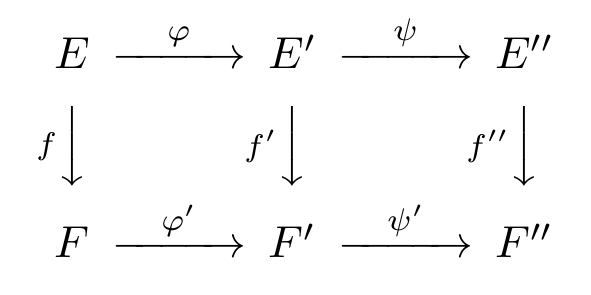
\includegraphics[scale=0.4]{image1.png}
		\end{center}
	
		On suppose que $f^{\prime} \circ \varphi=\varphi^{\prime} \circ f$, $f^{\prime \prime} \circ \psi=\psi^{\prime} \circ f^{\prime}$, $\operatorname{Im} \varphi=\operatorname{Ker} \psi$ et $\operatorname{Im} \varphi^{\prime}=\operatorname{Ker} \psi^{\prime}$.
		\begin{enumerate}
			\item Montrer que si $\varphi^{\prime}, f$ et $f^{\prime \prime}$ sont injectives alors $f^{\prime}$ l'est aussi.
			\item Montrer que si $\psi, f$ et $f^{\prime \prime}$ sont surjectives alors $f^{\prime}$ l'est aussi.
		\end{enumerate}
			\centering\rule{1\linewidth}{0.6pt}\end{exo}
		
		
		
		\begin{exo}\textbf{(****)}\quad\\[0.2cm]
			Soit $E$ un espace vectoriel de dimension finie, $u \in \mathscr{L}(E)$ nilpotent d'indice $p$ (tel que $u^{p}=0_{\mathscr{L}(E)}$ et $u^{p-1} \neq$ $\left.0_{\mathscr{L}(E)}\right)$ et $\Phi: v \in \mathscr{L}(E) \mapsto u \circ v-v \circ u$.
			
			\begin{enumerate}
				\item Montrer que, pour tout $n \in \mathbb{N}$ et tout $v \in \mathscr{L}(E)$,
				
				$$
				\Phi^{n}(\nu)=\sum_{k=0}^{n}(-1)^{k}\left(\begin{array}{l}
				n \\
				k
				\end{array}\right) u^{n-k} \circ \nu \circ u^{k} .
				$$\quad\\[0.4cm]
				
				\item Montrer que $\Phi$ est nilpotente et majorer son indice de nilpotence.
				\item Soit $a \in \mathscr{L}(E)$. 
				
				Montrer qu'il existe $b \in \mathscr{L}(E)$ tel que $a \circ b \circ a=a$.
				\item En déduire l'indice de nilpotence de $\Phi$.
	
			\end{enumerate}
			
			\centering\rule{1\linewidth}{0.6pt}\end{exo}
		
		
		
\end{minipage}\end{minipage} 



\end{document}